\documentclass[journal,11pt]{IEEEtran}

\usepackage{eurosym}
\usepackage{amsmath}
\usepackage{graphicx}
\usepackage{caption}

% correct bad hyphenation here
\hyphenation{op-tical net-works semi-conduc-tor}


\begin{document}
\title{Project 1: Report on Electricity Market Game}

\author{Sean~Jennings,~\IEEEmembership{Student Member,~IEEE}}

\markboth{ECEN 5427 -- Spring 2025}{}

\maketitle

\begin{abstract}
The abstract goes here.
\end{abstract}

% Note that keywords are not normally used for peerreview papers.
% \begin{IEEEkeywords}
% IEEE, IEEEtran, journal, \LaTeX, paper, template.
% \end{IEEEkeywords}

% \IEEEpeerreviewmaketitle

\section{Introduction}
\IEEEPARstart{T}{his} report details findings from the "Electricity Market Game" (EMG) project.
It begins with an overview of the major events that occurred in the game, 
subsequently documents our team's strategy for making bidding, investment, and retirement decisions.
We finish by explaining the major insights gained into long-term and short-term market dynamics,
highlighting the differences from real-world electricity markets.

\section{Team Strategy}

Conceptally, the strategy for the EMG can be broken into two major components that can be considered
separately:
\begin{enumerate}
  \item Bid strategy
  \item Planning strategy
\end{enumerate}

The bidding portion of the game emulates the operational aspects of an electricity market, with
a bid sheet submitted each round (a simulated year). By planning portion, we refer to components of the game
involving long-term decisions, run their course over many rounds (years). We will group both investment
and retirement of power plants into this broader "planning" category, since the decisions are closely
coupled.

Initially, we approached the bidding and planning aspects of our strategy as largely independent. 
As the game progressed, we realized that a joint bidding/investment strategy could be possible, although
we retained our initial strategy.

\subsection{Bid Strategy}

We settled on the relatively straightforward strategy of bidding at the marginal cost of fuel, with an extra multiplicative
factor. Prior to the first round, we debated whether bids should include an amortized value of fixed costs (the cost of loans and fixed O\&M),
before settling on a purely marginal cost-based approach.

The fuel costs $c_f$ for each fuel type were computed on a per MWh basis by accounting for the per unit fuel cost $\gamma$ (\texteuro / fuel unit),
the fuel density $\rho$ (MJ / fuel unit), and the thermal efficiency $\eta$ (unitless) via the following relation:
\begin{equation}
    c_f = 3,600 \frac{\gamma \eta}{\rho} \text{ [\texteuro/MWh]}.
\end{equation}
(The factor of 3,600 is due to the unit conversion 3,600 MJ = 1 MWh.)

The logic behind this strategy became apparent as the initial rounds progressed. As long as the market clearing
price is greater than or equal to the fuel costs, an accepted bid will generate revenue for the utility. Since
fixed costs are incurred regardless of whether or not the power plant is producing electricity, these are a sunk cost
with respect to the round-to-round bidding. Any revenue is better than none! But the market clearing price (MCP) is only
equal to the bid price for the generator that sits at the very top of the dispatch stack. So it is still possible
to recoup fixed costs, if the MCP is sufficiently high.

On the other hand, a company that bids higher than their marginal cost of operation can potentially be pushed "out of the money",
undercut by a competitor. Once a power plant is out of the money, it generates no revenue at all. Thus, there is an incentive
to bid as low as possible (while still operating with a profit).

For the first few rounds, we experimented with multiplying the marginal costs by some factor slightly greater than 1; typically, between 1.1 and 1.3.
However, we observed that some plants, particularly the natural gas plants, were falling out of the money from this approach. So we ended up removing the
factor and just using marginal costs directly.

\subsubsection{Carbon Tax}

Once the carbon tax was enacted, we incorporated it into our bidding price, effectively passing the cost of the carbon tax to the consumers of Etopia.
For each fuel type, we computed the per MWh price of carbon $c_{CO_2}$ based on the fuel's emissions factor $\epsilon$ (ton CO$_2$ / fuel unit), energy density $\rho$ (MJ / fuel unit)
and the carbon tax rate $\tau$ (\texteuro / ton CO$_2$) via equation
\begin{equation}
  c_{CO_2} = 3,600 \tau \epsilon / \rho  \text{ [\texteuro / MWh]}
\end{equation}



\subsection{Planning Strategy: Quantitative Aspects}

We began the game by evaluating the lifetime returns of each generation technologies to determine which would be the most profitable.
The lifetime profit $P$ (M\texteuro/MW) was computed on a per MW basis:
\begin{equation}
  P = C + t_\ell (R - E)
\end{equation}
where $C$ (M\texteuro/MW) is the total capital investments, $t_\ell$ is the expected lifetime (in rounds), $R$ is the revenue (M\texteuro/MW/round), and $E$ is the expenditures (M\texteuro/MW/round).

Capital costs were computed based on the price down payments $D$, yearly loan payments $L$, and the debt payback period $t_d$ via
\begin{equation}
  C = D + L \cdot t_d
\end{equation}

The yearly expenditures $E$ were calculated based on the fixed O\&M costs $E_0$ , the expected capacity factor $\alpha$, and an estimated average fuel cost $c_f$
(in \texteuro/MWh):
\begin{equation}
  E = E_0 + c_f \cdot \alpha \cdot T_y \text{ [M\texteuro/MW/round]}
\end{equation}
where $T_y = 8760$ is the number of hours in a year.


The expected yearly revenue is similarly based on the number of hours $T$ per year it runs, but also the electricity price $p_e$:
\begin{equation}
  R = \frac{10^6 \text{\texteuro}}{M\text{\texteuro}}  p_e \cdot \alpha \cdot T_y \text{ [M \texteuro /MW]}
\end{equation}

There is uncertainty in a number of these lifetime quantities. In particular, the fuel cost $c_f$, the electricity price $p_e$, and the number of operating hours per year $\alpha$
are all uncertain. To understand the range of possiblilities, we computed the electricity price which would be required to break even over the lifetime (i.e. setting $P=0$). 
Solving the previous equations for $p_e$, yields the following result:
\begin{equation}
  p_e = c_f + \frac{1}{\alpha \cdot T_y} (\frac{C}{t_\ell} + E_0)
\end{equation}

We estimated $c_f$ by simply taking an average over historical fuel prices. The capacity factor is the most complex to estimate, since it depends the following: 
the reliability coefficient $r$ (probability that the plant is down for maintainance), the renewable availability factor $\beta$ (for non-renewables $\beta=1$), and the market viability $\mu$,
via the equation:
\begin{equation}
  \alpha = r \cdot \beta \cdot \mu
\end{equation}

By market viability, we mean that percentage of the time which the generator is "in the money". This depends in the short-term on the bids that the other teams submit, 
and in the long-term on their capacity expansion plans. Since this is particularly difficult to estimate, we simplified the situation by considering the following scenarios:
1) the generator runs only during peak and shoulder hours ($\mu=1-5000/8760=0.429$) and 2) the generator runs during all hours ($\mu=1$).

Table \ref{tab:power_data} shows the results of this computation. This data illustrates how much of the breakeven price can be contributed to fixed versus variable 
costs. For example, a large portion of OCGT natural gas plants is the fuel costs, indicating a strong sensitivity to the fuel price. This levelized view of the energy
prices allows a fair comparison between renewable and non-renewable technologies.  We see that solar is the cheapest generation technology by a large margin.

\begin{table*}[h]
  \centering
  \begin{tabular}{lcccccc}
      \hline
      Type & $C$ (M\texteuro/MW) & $t_\ell$ (rounds) & $\beta$ & $c_f$ (\texteuro / MW) & $p_e$ (all hours, [\texteuro/MWh]) & $p_e$ (peak and shoulder-only, [\texteuro/MWh]) \\
      \hline
      Solar & 0.58 & 25 & 0.30 & 0.00 & 17.69 & 41.23 \\
      Wind & 1.79 & 25 & 0.59 & 0.00 & 25.23 & 58.82 \\
      Biomass & 1.80 & 40 & 1.00 & 18.09 & 39.66 & 68.38 \\
      Nuclear & 8.90 & 50 & 1.00 & 4.28 & 40.31 & 88.25 \\
      PowderCoal & 1.69 & 40 & 1.00 & 24.42 & 44.48 & 71.18 \\
      NaturalgasCCGT & 0.83 & 30 & 1.00 & 34.42 & 45.53 & 60.32 \\
      NaturalgasOCGT & 0.58 & 30 & 1.00 & 53.42 & 58.93 & 66.27 \\
      \hline
      Nuclear (purchased) & 2.425 & 26 & 1.00 & 26.27 & 55.54
  \end{tabular}
  \caption{Projections for Fuel Costs and Breakeven Electricity Prices estimated at Round 9}
  \label{tab:power_data}
\end{table*}

However, there are several limitations of this viewpoint. First, it provides only an average electricity cost, which does not account for the variability between
off-peak and peak markets, nor the variability between years. In particular, as an increasing portion of the grid is inundated with solar and wind, the round-to-round variability
in their availabilities will induce a round-to-round price variability. Indeed, we observe this price volatility in the later rounds of the game, as seen in Figure \ref{fig:prices}.
When renewable availability is high, the electricity prices will be lower and vise-versa. Given the
aforementioned uncertainties, we used these breakeven prices to help inform a more qualitative approach, described in the next section.  

\begin{center}
  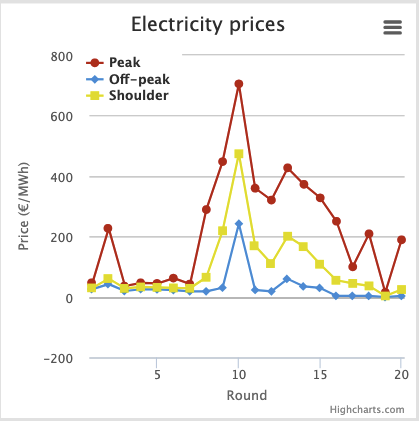
\includegraphics[width=0.9\linewidth]{Images/electricity_prices.png}
  \captionof{figure}{Electricity Prices over the EMG}
  \label{fig:prices}
\end{center}

\subsection{Planning Strategy: Qualitative Aspects}


From an investment standpoint, we began the game with a wait-and-see approach, trying to get a sense of the market dynamics before making any major
decisions.  Of course, Dominion Energy immediately made very large investments in wind and solar starting in the first round. Given that the grid-wide solar
and wind capacity was greatly increased, we saw an opportunity in non-intermittent baseload power. Given the zero-marginal cost of renewables, we expected
low prices in rounds where solar and wind were plentiful, and higher prices in rounds where solar and wind availability was lower. We were debating
construction of a second biomass plant when Dominion put its nuclear plant up for sale in Round 5. We knew we were getting a good deal on the plant (see Table \ref{tab:power_data}), since
it only had a six years of loans remaining and since Dominion was out of cash and forced to sell. However, given that electricity prices were quite low, it was
actually a somewhat risky decision. We ran a cash flow analysis to determine whether we'd be able to pay off the remaining several years of nuclear loans before
running out of cash. However, the uncertainty in future prices and aggregated capacity factor (amount of time each plant was "in the money") made it impossible
to know exactly.

With all the new solar and wind generation online at this point, electricity prices were quite low and we noticed that all the natural gas plants had
very low capacity factors, only running during peak and infrequently during shoulder hours. Despite being at the end of their loans (or very close),
the revenue from these markets was not enough to cover even the fixed O\&M costs. Furthermore, the prices of natural gas increased quite a bit during
these rounds (9-15), reducing their value even further. We retired two of our four natural gas plants in rounds 5 and 6, as we were preparing for
the nuclear purchase and the last two in rounds 11 and 13.

Fortunately, we were able to avoid defaulting on our nuclear debts, largely due to the spike in electricity prices beginning in round 8. It seems that other
teams were also feeling the price squeeze of Dominion's initial renewables grab, since a significant amount of system-wide generation was retired between rounds 5 and 9
(see Figure \ref{fig:system-wide-cap}).
After paying off the nuclear loans, we expected to have more cash on hand from nuclear revenue and therefore planned to invest in the renewable market
in later rounds. In the end, the nuclear bet paid off and we purchased both solar and wind generation in rounds 13, 16, and 22.

\subsection{Joint Bid and Planning Strategies}
I had the realization after a few rounds that it could be possible to consider the bidding and planning strategies together. For instance, if one
particular company had sufficient market share and cash, it could bid lower than marginal costs and operate at a loss in an attempt to drive competitors out of business.
Since all companies began with the same amount of cash, this wasn't initially applicable. But in the rounds after Dominion made its large investment,
all the other companies, ConEd included, had some incentive for prices to remain low and prevent Dominion from cornering the entire market.

This realization didn't set in until many rounds into the game, so we never incorporated any such multi-round bidding strategies and continued with the strategy described above.


\section{Insights Into Market Dynamics}

Various aspects of the market dynamics were discussed in situ with our Team strategy, but here we will highlight a few more pertinent points.
Figure \ref{fig:system-wide-cap} shows the tumultuous history of system-wide capacity investment and dismantling decisions, aggregated across all teams.
This plot demonstrates an inverted relationship with the fluctuations as prices (Figure \ref{fig:prices}). As predicted by basic economics: as supply increases, prices will decrease.
As a point of comparison, the total shoulder hour demand in round 1 was <11 GW, so the \~8GW investment by Dominion represented an additional investment of sizeable fraction of the entire
system size. While not all this capacity is "firm" (say \~3-4GW when accounting for renewable availability), it still far outpaces demand growth which was typically between -2 to 4 \%.



\begin{center}
  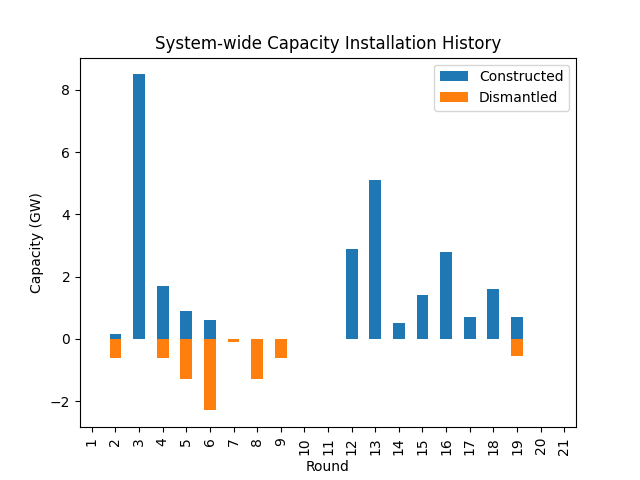
\includegraphics[width=0.9\linewidth]{Images/cap_install.png}
  \captionof{figure}{System-wide Installation History}
  \label{fig:system-wide-cap}
\end{center}

This demonstrates that an entirely free market does not necessarily make any gaurantees on price volatility, nor energy availability: there were a number of rounds where
electricity consumption decreased significantly to accomodate the inavailability of capacity. 
The massive investment in renewables effectively pushed all the other generation technologies out of the market. Even though regulatory intervention was required to avoid bankruptcy, in
the end, the result was an accelerated path towards carbon neutrality.

It would have been interesting to see this effect of zero-marginal-cost renewables pushing out other generation sources over an even longer time frame. As a thought experiment,
imagine the limit case where the entire grid is formed entirely of renewable sources. Then, assuming all market players assume a strategy of bidding at marginal cost, the electricity
price will be zero, and all utilities will eventually run out of money covering their fixed costs without revenue. It follows that a fully renewable grid operated under a market system
does not have an stable equilibrium point. Under this (radically simplified) model of electricity markets, if there is a stable equilibrium point, it must contain to some extent form of
baseload generation which can help raise electricity prices.

\section{Differences from Real-World Electricity Markets}

There are quite a few differences between the EMG and real-life energy markets. Some were already alluded to in previous sections, but to explicit list a few:
\begin{enumerate}
  \item Lack of a spot market
  \item Elasticity of demand / lack of capacity markets
  \item Renewable availability skirts operational considerations
\end{enumerate} 

While the game technically had a mechanism for spot markets, renewability availability and fuel prices were fully known prior to the start of the round. Thus,
bids could be made with perfect accuracy. In the EMG, it is entirely disadvantagous to bid less than your available capacity, so in effect the spot 
market was rarely a factor, except in cases of human error.  In real life, forecasts never align with reality so spot markets are much less trivial.

In real-world markets, unserved demand is treated much more stringently than simply applying an elasticity constant. Capacity and reserve markets help to ensure
that critical demands are served by introducing an incentive for building spare capacity.

Finally, simply adding a stochastic availability factor to renewable resources avoids some of the difficult operational questions which intermittency introduces. Maybe this approximation
holds true when restricting to generation stacks with low renewable penetrations. But as renewable penetrations increase it becomes an increasingly poor estimate. Particularly, a
grid formed with entirely renewable resources cannot meet a demand curve (at a reasonable cost) if the generation and demand profiles are sufficiently misaligned. Imagine a fully solar
grid with only night-time loads as a simple counterexample. The value of energy storage and arbitrage is neglected in our simplified model.


\section{A Successful Game?}

Evaluating whether the EMG was a success depends on the success criteria. If we are to consider whether or not the consumer of Etopia were delivered reliable electricity at a reasonable
price, it's not clear that this was the case. Electricity prices spiked abruptly and load was "shed" to avoid to handle inadequate system-wide capacity. While this eventually came
somewhat under control for off-peak and shoulder pricing, peak prices continued to spike near 200 \texteuro/MWh even in the game's final rounds.

The game was successful in terms of demonstrating a possible path towards a carbon neutral grid. In our case, low prices for zero-carbon technologies, competitive incentive, and a bit
of regulatory bailout were enough to push the grid to very low carbon emissions.

\section{Peer Review}

Overall, our team worked well together. Marco took the lead on submitting bid sheets in a timely manner. Joe did some great work on some of the forecasting, particularly in evaluating
whether the cash flow of the nuclear plant was feasible. I also repeated some of the breakeven projection so that we could compare and make sure they lined up. Madhura and Jordan both
contributed insights into the group discussion.















% \appendices
% \section{Proof of the First Zonklar Equation}
% Appendix one text goes here.
% 
% % you can choose not to have a title for an appendix
% % if you want by leaving the argument blank
% \section{}
% Appendix two text goes here.
% 
% 
% % use section* for acknowledgment
% \section*{Acknowledgment}
% 
% 
% The authors would like to thank...
% 
% 
% % Can use something like this to put references on a page
% % by themselves when using endfloat and the captionsoff option.
% \ifCLASSOPTIONcaptionsoff
%   \newpage
% \fi



% trigger a \newpage just before the given reference
% number - used to balance the columns on the last page
% adjust value as needed - may need to be readjusted if
% the document is modified later
%\IEEEtriggeratref{8}
% The "triggered" command can be changed if desired:
%\IEEEtriggercmd{\enlargethispage{-5in}}

% references section

% can use a bibliography generated by BibTeX as a .bbl file
% BibTeX documentation can be easily obtained at:
% http://mirror.ctan.org/biblio/bibtex/contrib/doc/
% The IEEEtran BibTeX style support page is at:
% http://www.michaelshell.org/tex/ieeetran/bibtex/
%\bibliographystyle{IEEEtran}
% argument is your BibTeX string definitions and bibliography database(s)
%\bibliography{IEEEabrv,../bib/paper}
%
% <OR> manually copy in the resultant .bbl file
% set second argument of \begin to the number of references
% (used to reserve space for the reference number labels box)
% \begin{thebibliography}{1}
% 
% \bibitem{IEEEhowto:kopka}
% H.~Kopka and P.~W. Daly, \emph{A Guide to \LaTeX}, 3rd~ed.\hskip 1em plus
%   0.5em minus 0.4em\relax Harlow, England: Addison-Wesley, 1999.
% 
% \end{thebibliography}

% biography section
% 
% If you have an EPS/PDF photo (graphicx package needed) extra braces are
% needed around the contents of the optional argument to biography to prevent
% the LaTeX parser from getting confused when it sees the complicated
% \includegraphics command within an optional argument. (You could create
% your own custom macro containing the \includegraphics command to make things
% simpler here.)
%\begin{IEEEbiography}[{\includegraphics[width=1in,height=1.25in,clip,keepaspectratio]{mshell}}]{Michael Shell}
% or if you just want to reserve a space for a photo:

% \begin{IEEEbiography}{Michael Shell}
% Biography text here.
% \end{IEEEbiography}
% 
% % if you will not have a photo at all:
% \begin{IEEEbiographynophoto}{John Doe}
% Biography text here.
% \end{IEEEbiographynophoto}
% 
% % insert where needed to balance the two columns on the last page with
% % biographies
% %\newpage
% 
% \begin{IEEEbiographynophoto}{Jane Doe}
% Biography text here.
% \end{IEEEbiographynophoto}

% You can push biographies down or up by placing
% a \vfill before or after them. The appropriate
% use of \vfill depends on what kind of text is
% on the last page and whether or not the columns
% are being equalized.

%\vfill

% Can be used to pull up biographies so that the bottom of the last one
% is flush with the other column.
%\enlargethispage{-5in}



% that's all folks
\end{document}


